\chapter{Euler Diagrams and Circuits}

\epigraph{Contrariwise, if it was so, it might be; and if it were so, it would be; but as it isn't, it ain't. That's logic.}{Lewis Carroll}

\begin{boxexample}{}{}
	Determine if this logic is valid. All students drink alcohol. Scott drinks alcohol. Therefor, Scott is a student.

	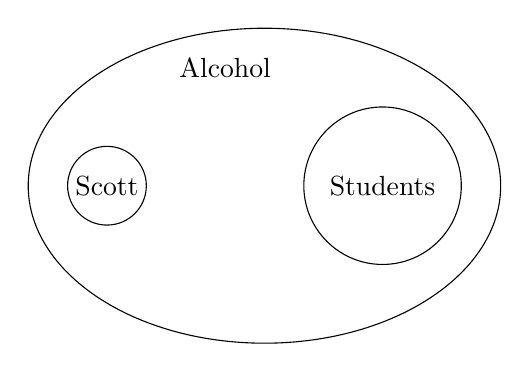
\begin{tikzpicture}
		\draw (0,0) ellipse (3 and 2);
		\node at (-.5,1.5) {Alcohol};
		\draw (1.5,0) circle (1);
		\node at (1.5,0) {Students};
		\draw (-2, 0) circle (0.5);
		\node at (-2,0) {Scott};
	\end{tikzpicture}

	This logic is invalid.
\end{boxexample}

\begin{boxexample}{}{}
	Determine if this logic is valid. All salespeople are annoying. Kelly is a salesperson. Therefor, Kelly is annoying.

	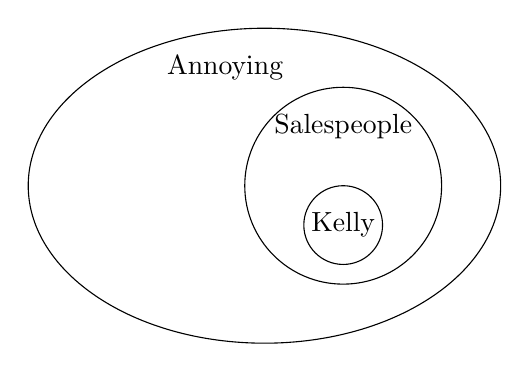
\begin{tikzpicture}
		\draw (0,0) ellipse (3 and 2);
		\node at (-.5,1.5) {Annoying};
		\draw (1,0) circle (1.25);
		\node at (1,0.75) {Salespeople};
		\draw (1,-.5) circle (0.5);
		\node at (1,-.5) {Kelly};
	\end{tikzpicture}

	This logic is valid.
\end{boxexample}

\begin{boxexample}{}{}
	Determine if this logic is valid. All teachers are nice. John is not nice. Therefor, John is not a teacher.

	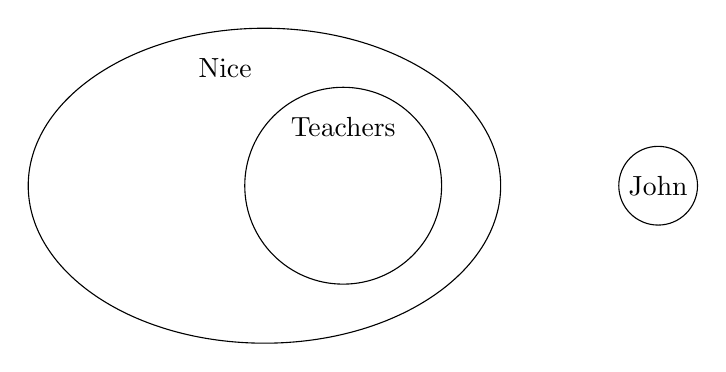
\begin{tikzpicture}
		\draw (0,0) ellipse (3 and 2);
		\node at (-.5,1.5) {Nice};
		\draw (1,0) circle (1.25);
		\node at (1,0.75) {Teachers};
		\draw (5,0) circle (0.5);
		\node at (5,0) {John};
	\end{tikzpicture}

	This logic is valid.
\end{boxexample}

\begin{boxexample}{}{}
	Write this curcuit as a statement.

	\begin{circuitikz}
		\draw (0,0)
		to [short, *-] (1,0)
		to [short] (1,1)
		to [short] (2,1)
		to [nos,l=P] (3,1)
		to [short] (4,1)
		to [nos,l=Q] (5,1)
		to [short] (6,1)
		to [short] (6,0)
		to [short] (7,0)
		to [nos,l=S] (8,0)
		to [short,-*] (9,0)
		(1,0)
		to [short] (1,-1)
		to [short] (2,-1)
		to [nos,l=R] (3,-1)
		to [short] (6,-1)
		to [short] (6,0);
	\end{circuitikz}

	\[
		((P \land Q) \lor R) \land S
	\]
\end{boxexample}
